\documentclass{article}

\usepackage{graphicx}

\setlength{\parskip}{\medskipamount}

\title{Advanced Object Oriented Programming and Design\\
\medskip
\large Theoretical Homework 1}
\author{Abraham Murciano and Daniel Klein}

\begin{document}

\maketitle

We are given the following code which we can assume is correct.

\begin{verbatim}
	public static void main(String[] args) {
	    int x;
	    String y;
	    C b1 = new B();
	    A[] arrA = new A[3];
	    arrA[0] = new B(x, y);
	    arrA[1] = new B();
	    arrA[2] = new C();
	    arrA[0].f();
	    arrA[0].g();
	    arrA[0].h();
	}
\end{verbatim}

\section*{Section A}

We are told A is an interface, and we are tasked with writing its declaration.

\begin{verbatim}
	interface A {
	    void f();
	    void g();
	    void h();
	}
\end{verbatim}

\section*{Section B}

We must now implement classes B and C.

\begin{verbatim}
	class C implements A {
	    void f() {}
	    void g() {}
	    void h() {}
	}

	class B extends C {
	    public B() {}
	    public B(int, String) {}
	}
\end{verbatim}

\section{Section C}

Below is a UML diagram for the classes A, B, and C.

\begin{figure}[htbp]
	\centering
	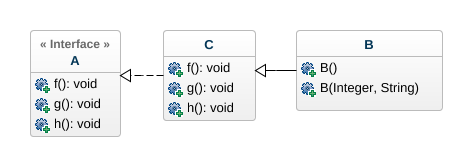
\includegraphics[width=\textwidth]{uml.png}
\end{figure}


\section{Section D}

C cannot be an interface, because we call its constructor in the code, and interfaces cannot be instantiated.

\end{document}